\subsection{Temps}
\label{section:temps}

Dans la section \ref{subsubsection:time}, nous avons pu voir qu'il est important de gérer le temps que l'application voit s'écouler. En section \ref{section:work:time}, nous avons présenté l'implémentation qui a été choisie pour résoudre cette problématique. Maintenant, nous souhaitons évaluer ses performances.

\subsubsection{Protocole expérimental}
L'objectif principal étant de montrer qu'il est possible de faire de la virtualisation légère, nous souhaitons mesurer le surcoût ajouté par cette interception lors de l'exécution de Simterpose. Notre expérience va donc consister à comparer les temps d'exécution d'une application utilisant Simterpose avec et sans interception via \texttt{LD\_PRELOAD}. Néanmoins, le changement de médiation ne devrait pas influer sur les performances réelles car chaque médiation intervient uniquement lorsqu'on souhaite effectuer des appels systèmes réseaux que l'on fasse de l'interception avec \texttt{LD\_PRELOAD} ou pas.

L'application qui a été créée pour effectuer nos expériences exécute différents appels à des fonctions temporelles (\texttt{ftime}, \texttt{time}, \texttt{gettimeofday}, \texttt{localtime}, \texttt{mktime}...). Le protocole utilisé consiste à exécuter 20 fois l'application puis une moyenne du temps d'exécution ainsi qu'une mesure des temps minimum et maximum sont calculés.

\subsubsection{Résultat}
 Notre expérience consiste à exécuter l'application qui effectue les appels temporels avec Simterpose sans \texttt{LD\_PRELOAD} et avec \texttt{LD\_PRELOAD}. Les résultats de l'expérience sont présentés Figure \ref{Temps_FM}. On constate que le temps d'exécution avec interception via \texttt{LD\_PRELOAD} est plus ou moins constant (environ 1,03 secondes), alors que celui sans interception varie énormément, entre 0,82 et 1,13 secondes. 

\begin{figure}[H]
  \centering
    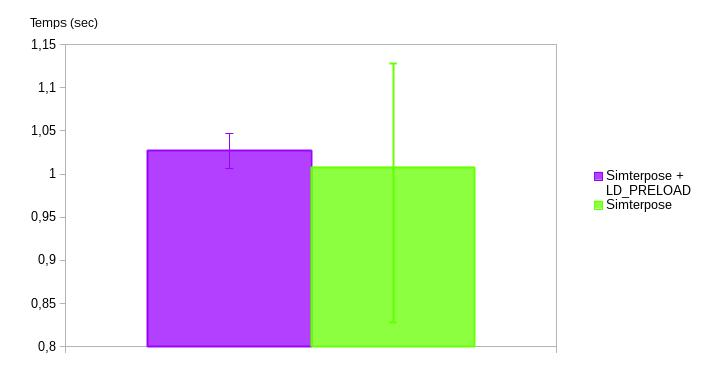
\includegraphics[scale=0.50]{mesures/graph/global_time.jpg}
    \caption{Temps d'exécution d'une application temporelle avec interception via \texttt{LD\_PRELOAD} et sans interception.}
    \label{Temps_FM}
\end{figure}

\subsubsection{Analyse}
Cela est dû au fait que lorsqu'on appelle des fonctions temporelles sans interception via \texttt{LD\_PRELOAD} la bibliothèque \texttt{VDSO} est appelée pour gérer l'appel et accéde elle-même à la mémoire. Néanmoins, en moyenne les deux expériences ont environ le même temps d'exécution, 1 seconde pour la première et 1,02 secondes pour la deuxième.

\subsubsection{Conclusion}
Pour conclure, cette exéprience nous permet de montrer que l'interception via \texttt{LD\_PRELOAD} a un surcoût négligeable lorsqu'on utilise Simterpose. Il est donc possible de mettre en place une virtualisation légère pour la gestion du temps.

%% \subsubsection{Address translation}
%% Nous allons maintenant voir s'il en est de même  lorsqu'on exécute l'application qui effectue les appels temporels avec Simterpose en \textit{address translation} avec et sans interception via \texttt{LD\_PRELOAD}. Les résultats cette expérience sont présentés Figure \ref{Temps_AT}. On constate ici aussi que le temps d'exécution avec interception via \texttt{LD\_PRELOAD} est plus ou moins constant (environ 1,02 seconde), alors que celui sans interception varie beaucoup, entre 0,86 et 1,12 secondes. Cela est dû comme précédement à l'utilisation de la bibliothèque \texttt{VDSO} en l'absence d'interception via \texttt{LD\_PRELOAD}. De plus, le temps d'exécution moyen des deux expériences est le même: 1,02 secondes. Dans ce cas, on peut dire que l'interceprtion via \texttt{LD\_PRELOAD} en \textit{address translation} n'a aucun surcoût.

%% \begin{figure}[H]
%%   \centering
%%     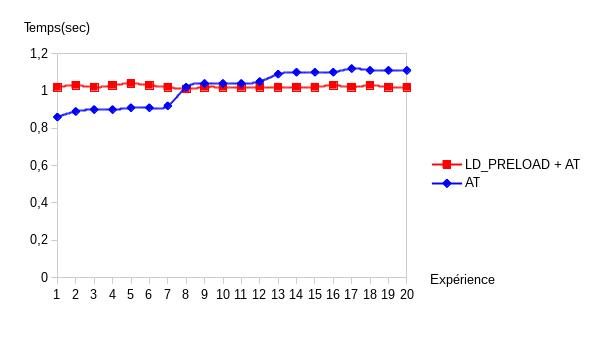
\includegraphics[scale=0.50]{mesures/graph/Temps_AT.jpg}
%%     \caption[Temps d'exécution d'une application temporelle en \textit{address translation}]{Temps d'exécution d'une application temporelle en \textit{address translation} avec interception via \texttt{LD\_PRELOAD} et sans interception.}
%%     \label{Temps_AT}
%% \end{figure}


%% Ainsi, nous avons pu voir que le surcoût dû à l'interception des fonctions temporelles via \texttt{LD\_PRELOAD} est inexistant en \textit{address translation} et qu'il est négligeable \textit{full mediation} (environ 2\%). On peut donc considérer que nous avons réussi à mettre en place une virtualisation légère qui gère également l'écoulement du temps et qui plus est de façon particulièrement efficace. De plus, en comparant les deux graphiques présentés Figure \ref{Temps_FM} et \ref{Temps_AT}, on voit bien que les courbes d'interception via \texttt{LD\_PRELOAD} se superposent et qu'il en est de même pour celles sans interception quelque soit la médiation utilisée. Le changement de médiation n'influe donc par sur les performances d'interception avec \texttt{LD\_PRELOAD}. Cela confirme l'hypothèse que nous avions fait.

\vspace{0.5cm}
